\documentclass[tikz, border=5mm]{standalone}

\begin{document}
 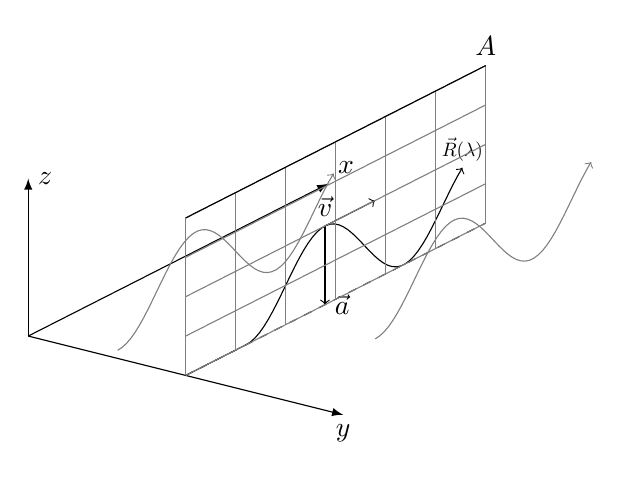
\begin{tikzpicture}[x={(1,-.25,0)}, y={(0,1,0)}, z={(.25,0,-1)}]
    % Axes
    \begin{scope}[->, >=latex]
      \draw (0,0,0) -- (4,0,0) node [below] {$y$};% x
      \draw (0,0,0) -- (0,2,0) node [right] {$z$};% y
      \draw (0,0,0) -- (0,0,6) node [above right] {$x$};% z
    \end{scope}

    % Plots
      \draw [dashed] (2,0,0) -- (2,0,6);
      \draw [<-] (2, 0, 2+pi/4) node [right] {$\vec{a}$} -- +(0,1,0);
      %\fill (2, 0, 2+pi/4) circle (2pt);
      \draw[-](2,0,0)--(2,0,2-pi/4);
      \draw [domain=-pi/4:3/4*1.5*pi, variable=\z, samples=50,->] plot (2, {.5+.5*sin(2*\z r)}, 2+\z) node[scale=0.7,above]
      {$\vec{R}(\lambda)$};
      \draw[->](2,1,2+pi/4) node[above]{$\vec{v}$} --+(0,0,1);

      \foreach \x in {0,1,...,6}{
      \draw[-,color=gray](2,0,\x)--(2,2,\x);
      }
      \foreach \x in {0,0.5,...,2}{
      \draw[-,color=gray](2,\x,0)--(2,\x,6);
      }
      \foreach \x in {1,3}{
       \draw [domain=-pi/4:3/4*1.5*pi, variable=\z, samples=50,->,color=gray,thin] plot (\x, {.5+.5*sin(2*\z r)}, \x+\z);
      }
      \draw[-] (2,2,0)--(2,2,6) node[above]{$A$};
    
  \end{tikzpicture}
\end{document}